\documentclass[tikz, border = 10pt]{standalone}

\usepackage{newpxtext,newpxmath}   % /upbeta
%\usepackage{fouriernc}            % /otherbeta
\usepackage{amsmath}
\renewcommand{\familydefault}{\sfdefault}
\usepackage{mathastext}

\usetikzlibrary{positioning, quotes, calc, math, arrows.meta, bending, shapes, backgrounds}

\tikzset{
every edge quotes/.style = {fill = white},
every node/.style = {scale = 1.1},
manifest/.style = {rectangle, draw, thin, inner sep = 3pt, minimum width = 1cm,
   minimum height = .85cm, align = center},
latent/.style = {ellipse, draw, thin, inner sep = 3pt, minimum width = 1cm,
   minimum height = .85cm},
residual1/.style = {circle, draw, thin, minimum size = 5mm, inner sep = 1pt},
residual2/.style = {rectangle, minimum width = 0.5pt, minimum height = 1.5mm,
   inner sep = 0pt, outer sep = 0mm},
regression/.style = {-{Stealth[length = 1.5mm]}, thin, shorten > = 1pt, 
   inner sep = 1.5pt, outer sep = 0mm},
covariance/.style={{Stealth[length = 1.5mm]}-{Stealth[length = 1.5mm]}, thin,
   shorten > = 1pt, shorten < = 1pt, inner sep = 1.5pt},
variance/.style={{Stealth[length = 1mm]}-{Stealth[length = 1mm]}, thin,
   shorten > = 1pt, shorten < = 1pt, inner sep = 1pt},
interaction/.style = {-{Stealth[sep = 1pt, length = 1.5mm] . Circle[length = 4pt]},
   thin, shorten > = -2pt},
constant/.style = {draw, thin, inner sep = 1pt, regular polygon,
   regular polygon sides = 3, minimum size = 5mm},
group/.style = {rectangle, inner sep = 2pt, minimum width = 15mm, minimum height = 5mm, 
   align = center}
}

\begin{document}
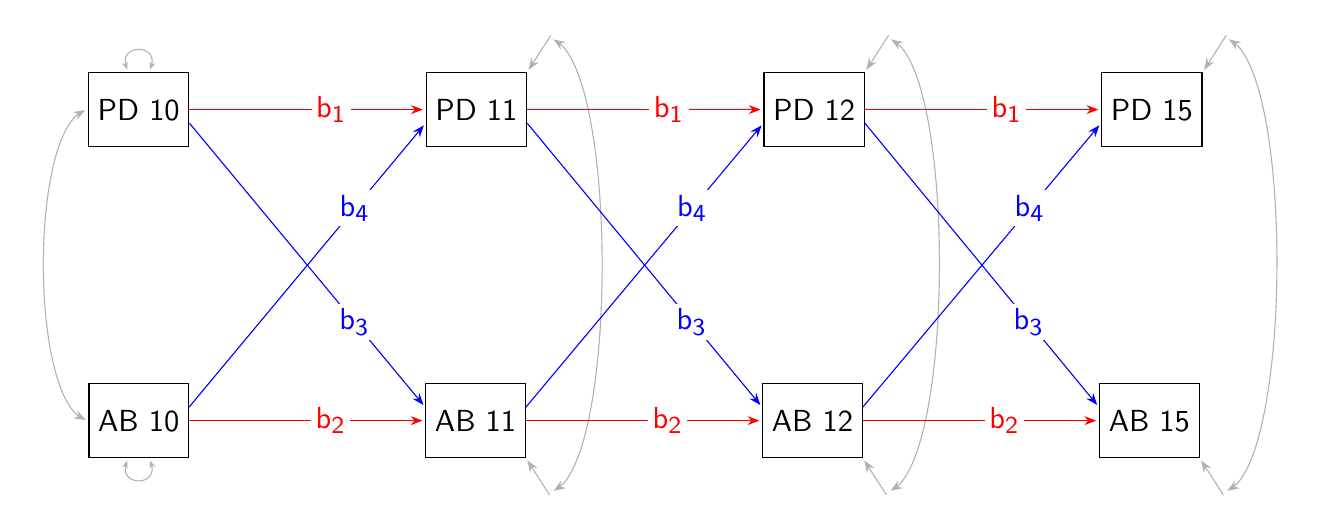
\begin{tikzpicture}

%% Manifest
\node [manifest] (x1) {PD 10};
\node [manifest] (x2) [right = 3cm of x1] {PD 11};
\node [manifest] (x3) [right = 3cm of x2] {PD 12};
\node [manifest] (x4) [right = 3cm of x3] {PD 15};

\node [manifest] (y1) [below = 3cm of x1] {AB 10};
\node [manifest] (y2) [right = 3cm of y1] {AB 11};
\node [manifest] (y3) [right = 3cm of y2] {AB 12};
\node [manifest] (y4) [right = 3cm of y3] {AB 15};

%% Regressions - Stability
\path [regression, red] (x1) edge ["$b_{1}$", pos = 0.6] (x2); 
\path [regression, red] (x2) edge ["$b_{1}$", pos = 0.6] (x3); 
\path [regression, red] (x3) edge ["$b_{1}$", pos = 0.6] (x4); 

\path [regression, red] (y1) edge ["$b_{2}$", pos = 0.6] (y2); 
\path [regression, red] (y2) edge ["$b_{2}$", pos = 0.6] (y3); 
\path [regression, red] (y3) edge ["$b_{2}$", pos = 0.6] (y4); 

%% Regressions - Cross-lagged effects
\path [regression, blue] (x1.345) edge ["$b_{3}$", pos = 0.7] (y2.165); 
\path [regression, blue] (x2.345) edge ["$b_{3}$", pos = 0.7] (y3.165); 
\path [regression, blue] (x3.345) edge ["$b_{3}$", pos = 0.7] (y4.165); 

\path [regression, blue] (y1.15) edge ["$b_{4}$", pos = 0.7] (x2.195); 
\path [regression, blue] (y2.15) edge ["$b_{4}$", pos = 0.7] (x3.195); 
\path [regression, blue] (y3.15) edge ["$b_{4}$", pos = 0.7] (x4.195); 

%% Exogenous variances and covariance
\path [variance, black!30] (x1.105) edge [bend left = 120, looseness = 4.5] (x1.75);
\path [variance, black!30] (y1.285) edge [bend left = 120, looseness = 4.5] (y1.255);
\path [covariance, black!30] (x1.180) edge [bend right = 80, looseness = 0.5] (y1.180);

%% Residuals ...
\node [residual2] (e2) [above right = 4mm and 3mm of x2] {};
\node [residual2] (e3) [above right = 4mm and 3mm of x3] {};
\node [residual2] (e4) [above right = 4mm and 3mm of x4] {};
\path [regression, black!30] (e2) edge (x2.north east);
\path [regression, black!30] (e3) edge (x3.north east);
\path [regression, black!30] (e4) edge (x4.north east);

\node [residual2] (e6) [below right = 4mm and 3mm of y2] {};
\node [residual2] (e7) [below right = 4mm and 3mm of y3] {};
\node [residual2] (e8) [below right = 4mm and 3mm of y4] {};
\path [regression, black!30] (e6) edge (y2.south east);
\path [regression, black!30] (e7) edge (y3.south east);
\path [regression, black!30] (e8) edge (y4.south east);

%% and their covariances
\begin{scope}[on background layer]
\path [covariance, black!30] (e2.260) edge [bend left = 75, looseness = 0.4] (e6.80);
\path [covariance, black!30] (e3.260) edge [bend left = 75, looseness = 0.4] (e7.80);
\path [covariance, black!30] (e4.260) edge [bend left = 75, looseness = 0.4] (e8.80);
\end{scope}

\end{tikzpicture}
\end{document}
